\chapter{Analysis}

This chapter will describe shortly the dataset provided for this task and discuss its challenges and problems. Then, an explanation will be given on how asbestos is detected in these images. The majority of the dataset was initially unlabeled and had to be labeled with the knowledge inferred from the provided ground truth set. The related work section gives a brief summary on the current work on asbestos detection, transfer learning on medical images as well as on general SEM images.

\section{Dataset}

%The dataset was generously provided by Microscan Service SA, which is a certified laboratory that specializes on scanning electron microscopy and microanalysis. It is located in Lausanne, Switzerland. They also provided a ground truth sample to show how asbestos looks like. The goal was to learn typical asbestos-like structures from the ground truth samples and then label the remaining images accordingly. Currently they analyze all the asbestos samples manually which is a time and cost intensive task.\\

The provided dataset consists of about 2'000 microscopic images with and without asbestos fibers. The images come in two different dimensions and different qualities. Most of the images are in the format of 1024x1024 pixels and using up 1.1 MB of disk space but some are in 1024x768 pixels and use only around 700 kB of disk space. The smaller images were originally in TIF format which needed to be converted into PNG format in order to load them into python objects. All images are in grey color space. Since all architectures have been originally trained on color images, the image is transformed into an RGB tensor during dataset preparation. All gray space values ranging from 0 to 255 are copied into each channel of RGB. In Figure~\ref{fig:chrysotile_classification} two very typical asbestos images are shown from the pre-labeld ground truth set.

\begin{figure}[h]
\centering
\caption{Two very typical examples of chrysotile (curly) asbestos. Detection is done visually by locating the fibrous strands.}
\subfigure{
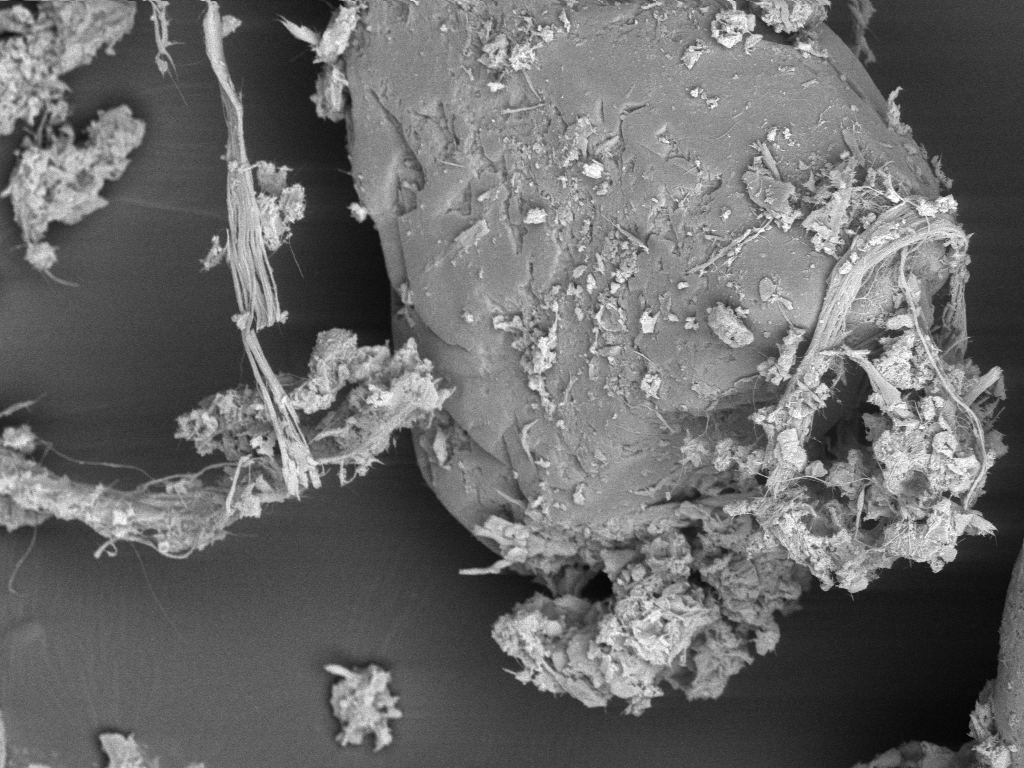
\includegraphics[width=.45\textwidth]{images/chapter2/howto/asbestos-042.png}
}
\subfigure{
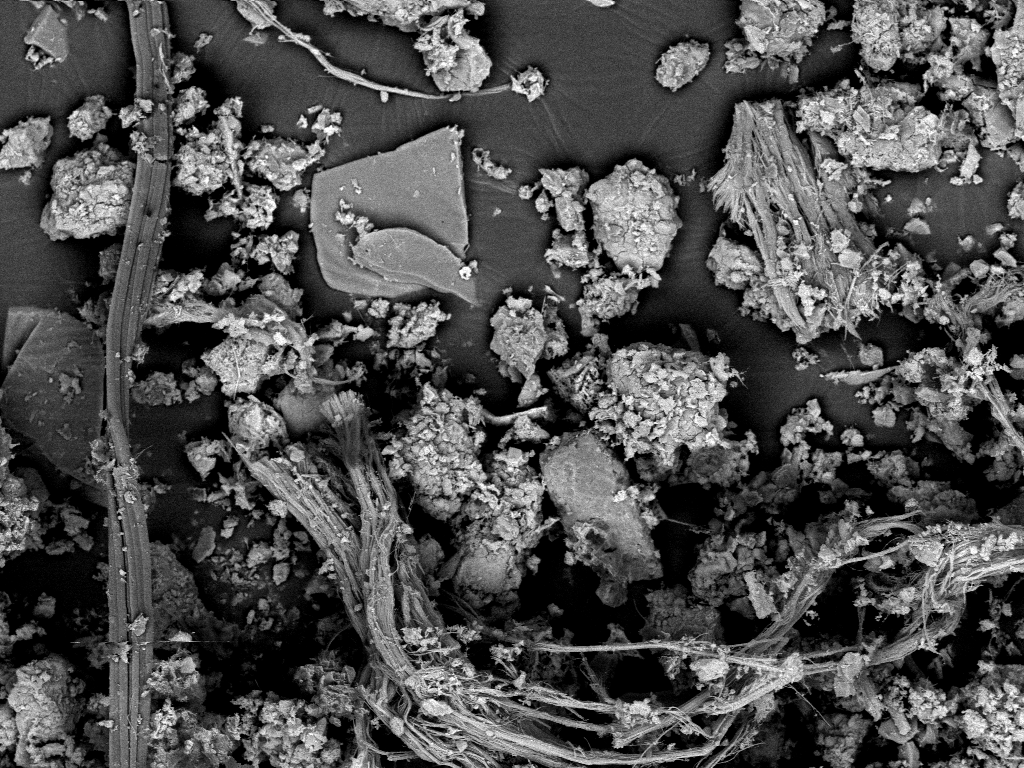
\includegraphics[width=.45\textwidth]{images/chapter2/howto/asbestos-105.png}
}
\label{fig:chrysotile_classification}
\end{figure}

Asbestos detection can be a very complex problem if  aspect ratio, length, density and count are included into classification in order to additionally decide if these asbestos samples pose a potential threat to human health. For this thesis' task, the detection of chrysotile asbestos fibers is sufficient regardless of their size. Of course some asbestos fibers are rather small and it is not clear if this actually is asbestos or not. Chrysotile fibers are more flexible than other types of asbestos which gives them the fibrous almost hair-like look in serpentinite rocks and under the microscope. They can be spun and woven into fabric and industrial products. The fibers can be more then 10 centimeters  long but in processed material they are much shorter. Chrysotile asbestos is also called curly asbestos because of its charateristic form. Detecting  them is simply looking at the image and finding these wooden-like fibrous strands which are composed of smaller bundles of fibrils. Often, as  seen in Figure~\ref{fig:chrysotile_classification}, the fibrils are spreading  from the bigger fibrous strands and make the detection easy. Other times only small fibrils are seen which makes it much harder to detect.

In Figure~\ref{fig:asbestos_examples} three images labeled as containing asbestos are shown whereas in Figure~\ref{fig:non-asbestos_examples} three images without asbestos are shown. These images are not from the pre-labeled ground truth but from the other unlabeled distribution, which come in a different quality and makes up the majority of all samples. \\

\begin{figure}[h]
\centering
\caption{Three examples of images \textbf{with asbestos fibers}. On the left, the asbestos fibers are clearly visible, in the middle it's much harder to find them. In the right image there might be none, although the image is labeled as having asbestos in it.}
\subfigure{
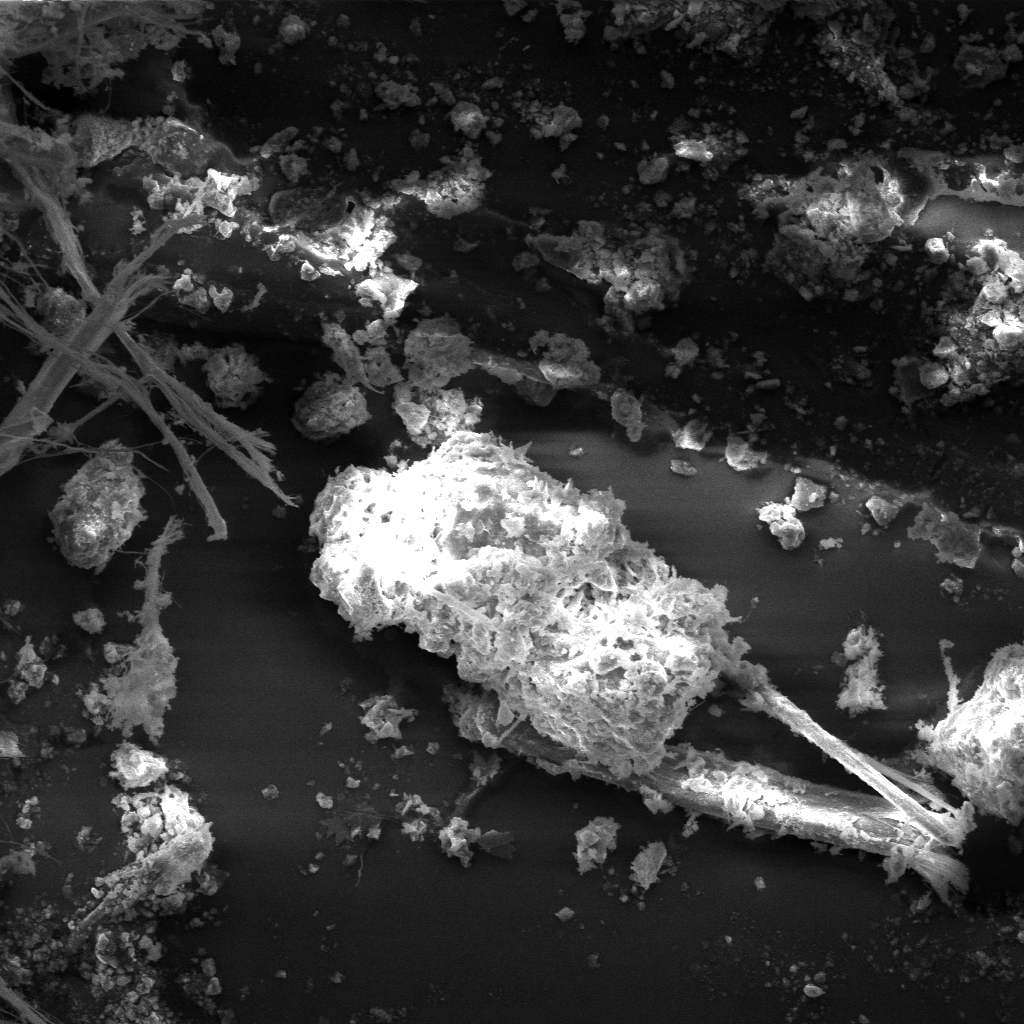
\includegraphics[width=.31\textwidth]{images/chapter2/asbestos_one.png}
}
\subfigure{
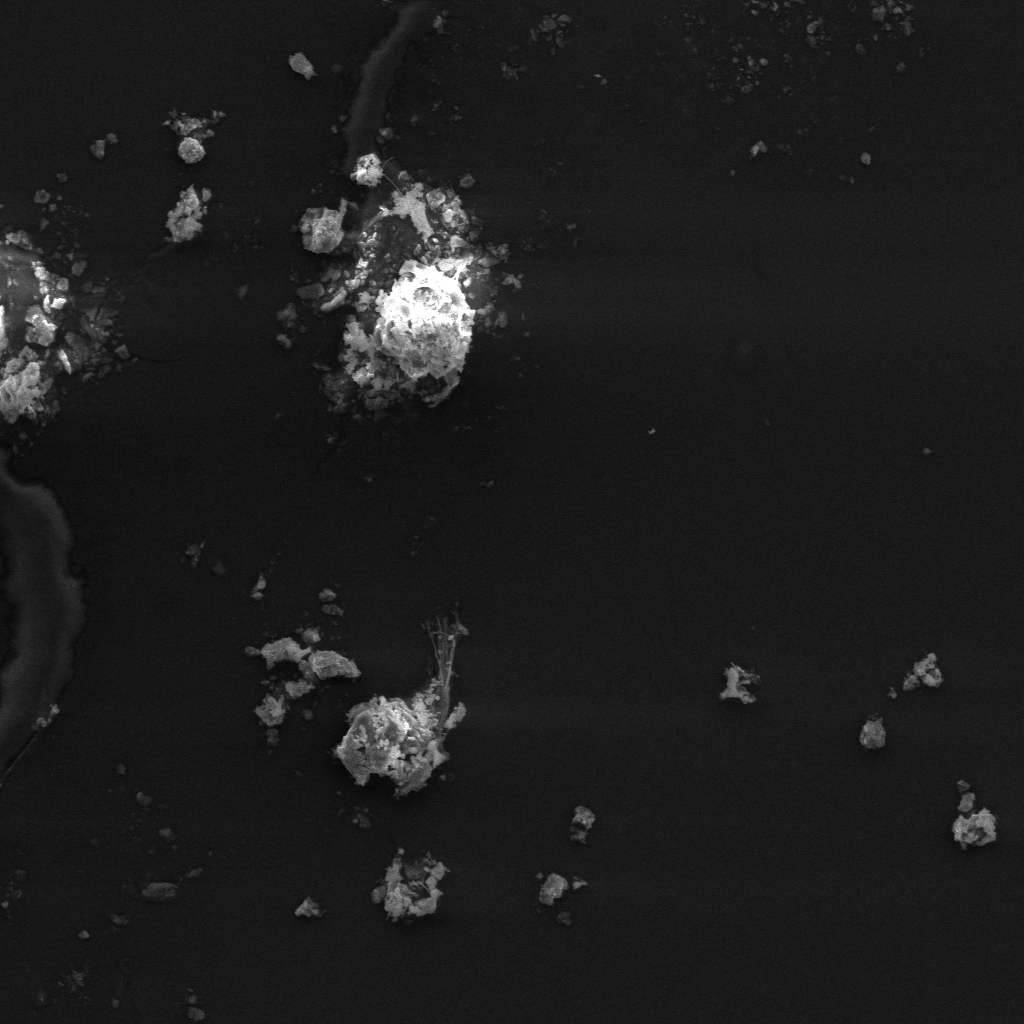
\includegraphics[width=.31\textwidth]{images/chapter2/asbestos_two.png}
}
\subfigure{
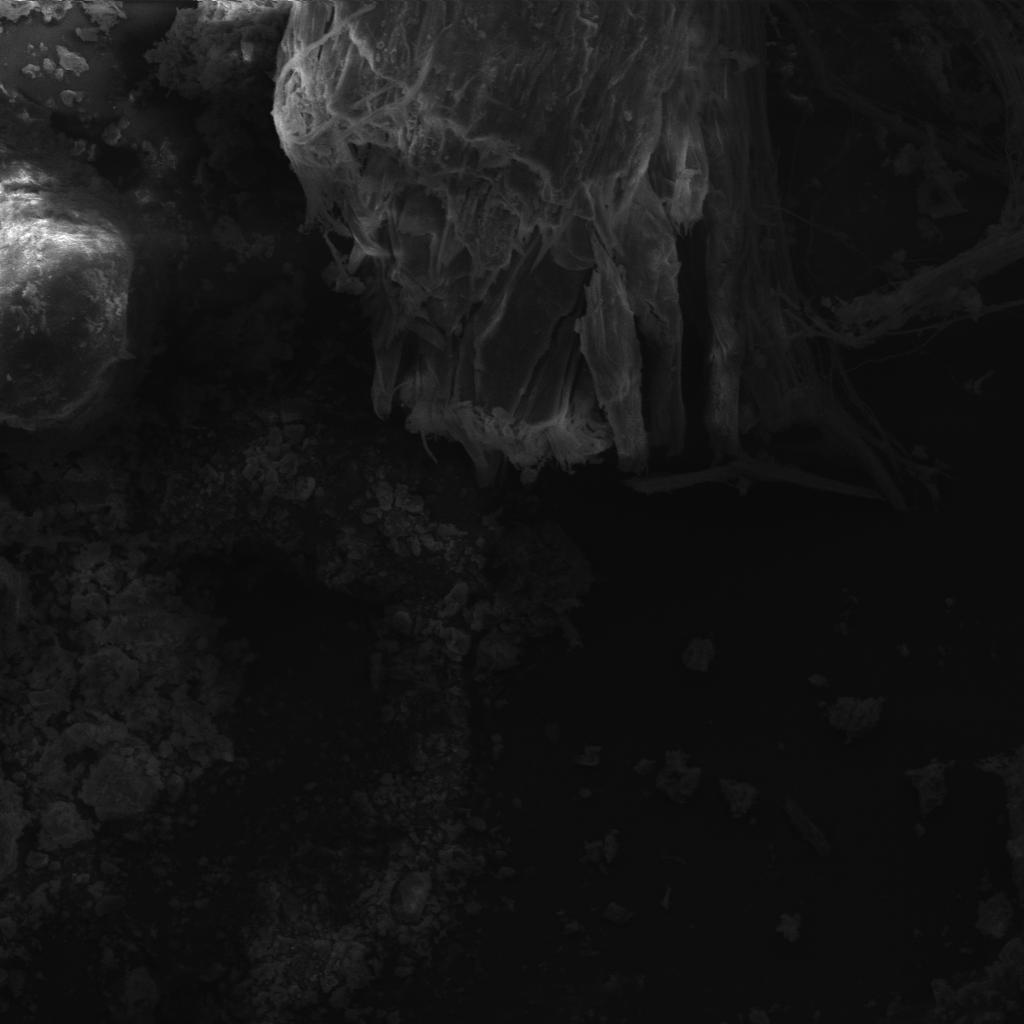
\includegraphics[width=.31\textwidth]{images/chapter2/asbestos_three.png}
} 
\label{fig:asbestos_examples}
\end{figure}

\begin{figure}[h]
\centering
\caption{Three examples of images \textbf{without asbestos fibers}. On the left image, there is clearly no asbestos to be found. In the middle and left image it's already much more difficult to be certain that there are no chrysotile fibers present.}
\subfigure{
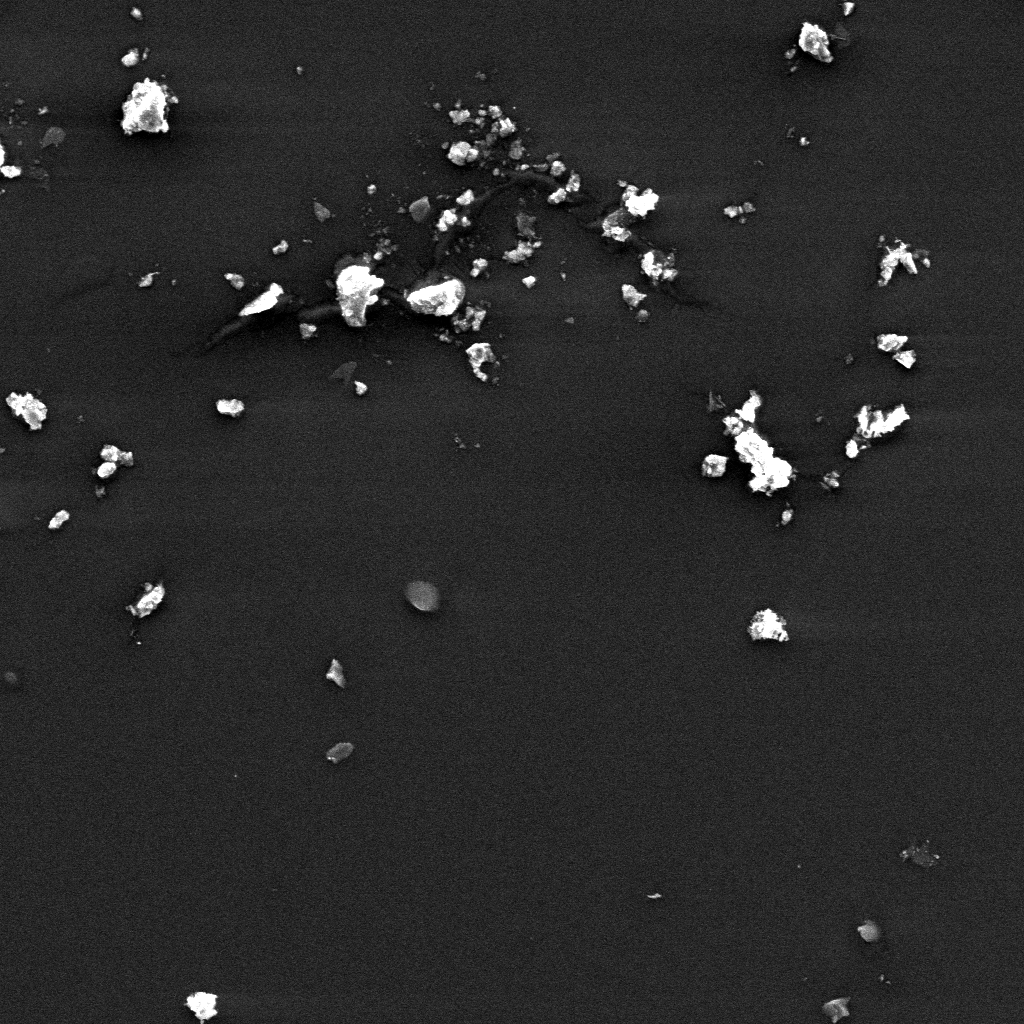
\includegraphics[width=.31\textwidth]{images/chapter2/non-asbestos_one.png}
}
\subfigure{
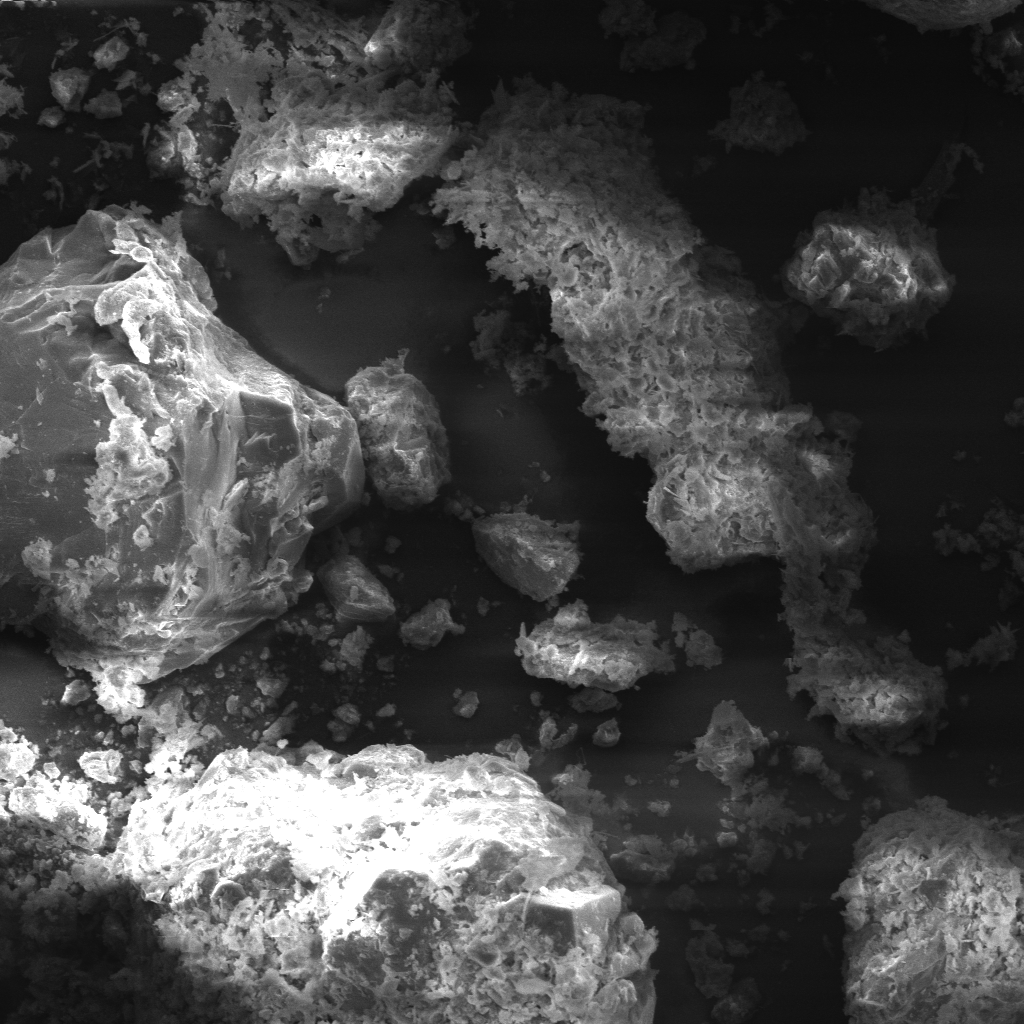
\includegraphics[width=.31\textwidth]{images/chapter2/non-asbestos_two.png}
}
\subfigure{
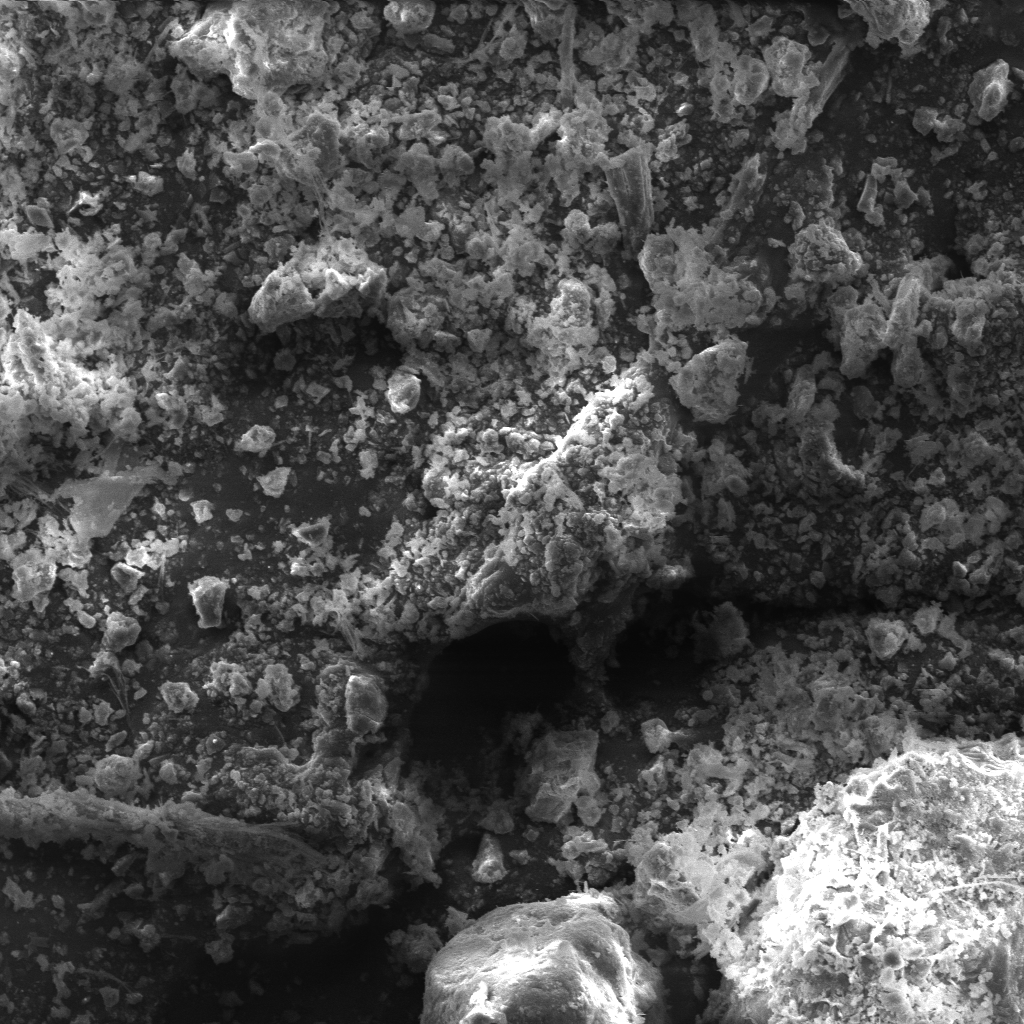
\includegraphics[width=.31\textwidth]{images/chapter2/non-asbestos_three.png}
}
\label{fig:non-asbestos_examples}
\end{figure}

With the dataset, a ground truth folder was provided with 116 images pre-labeled as having asbestos fibers in them or not. From these 116 images the remaining images needed to be manually labeled. Some of the later labeled images were checked by the laboratory but Figure~\ref{fig:wrong_asbestos_labeling} shows that even that leaves much space for errors.  According to the laboratory, the image shown in Figure~\ref{fig:wrong_asbestos_labeling} has no asbestos in it. Nonetheless, there are several areas where asbestos-like structures emerge once the image is made brighter with a photo-editing tool, especially a long fiber on the left side of the image becomes visible and is marked by two arrows. Brightening, sharpening and other simple editing tools are often used prior to classification to make the structures more visible. This is to show, that the labeled data for training will most certainly have errors in it and that some images might look like having asbestos fibers in them but actually don't and the other way around. In the laboratory, samples are examined with additional methods to be sure if asbestos is present or not, but that is not part of the master thesis. Therefore one of the main goals of this thesis is to be able to label all images and reduce the manual workload. Uncertain images should be labeled as containing asbestos and if needed examined further by the laboratory. That means that the rate of false negatives should be as low as possible.

\begin{figure}[h]
\centering
\caption{After brightening up the image and looking at it carefully, many different asbestos like structures emerge.}
\subfigure{
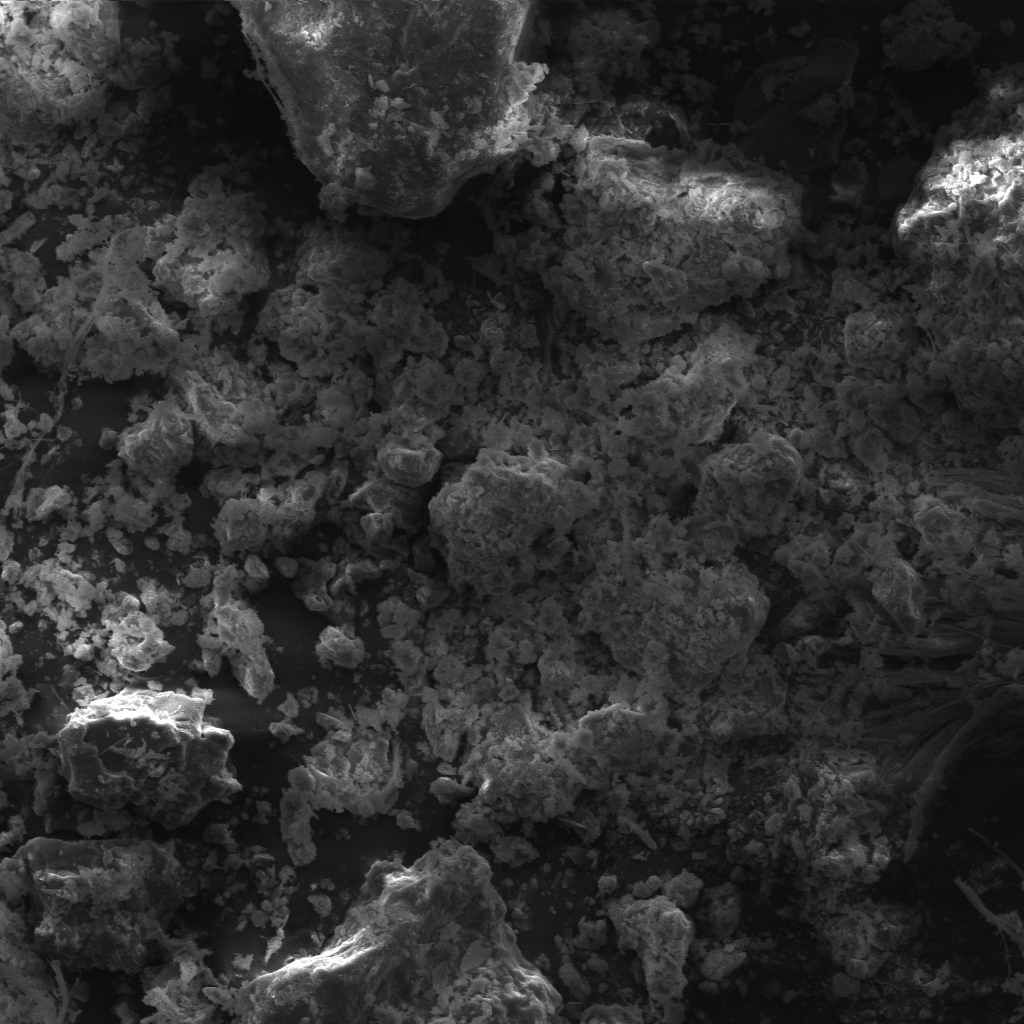
\includegraphics[width=.4\textwidth]{images/chapter2/probably_wrong_label.png}
}
\subfigure{
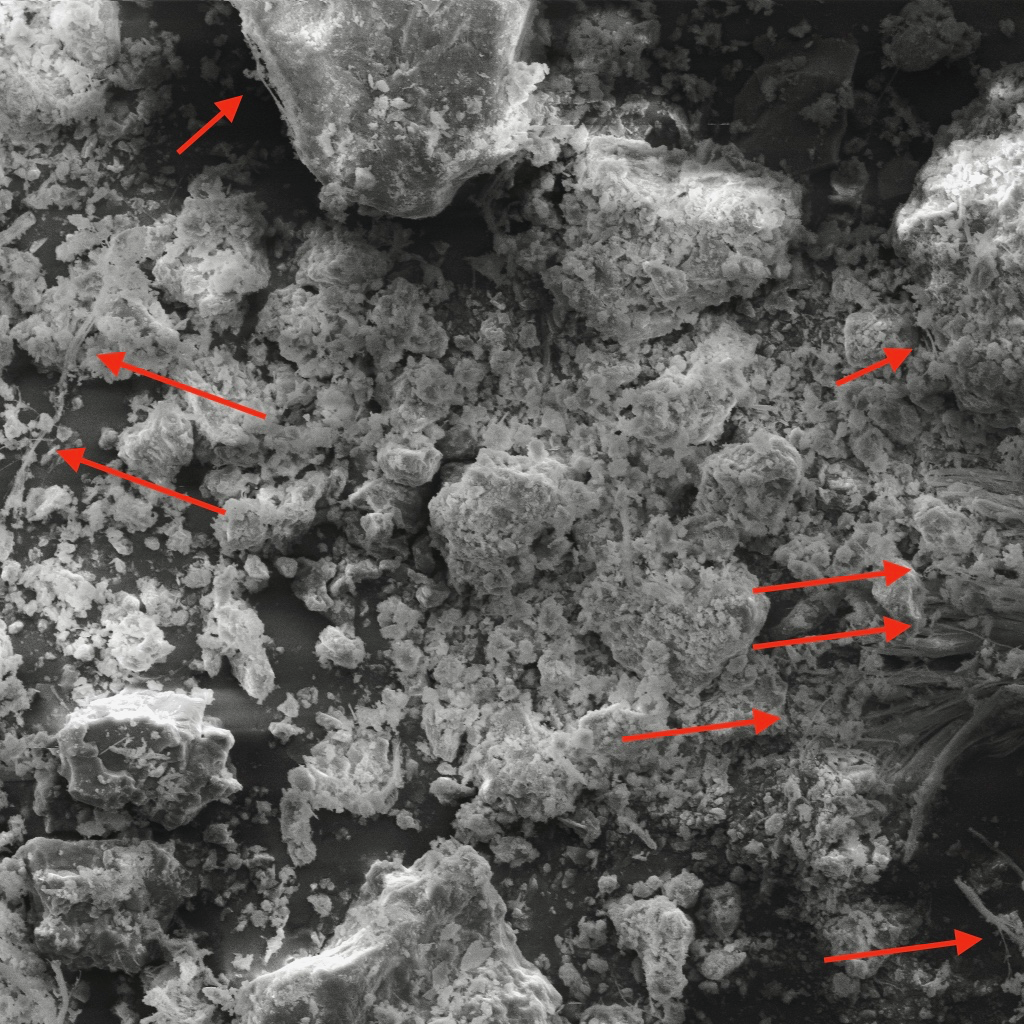
\includegraphics[width=.4\textwidth]{images/chapter2/probably_wrong_label_edited.png}
}
\label{fig:wrong_asbestos_labeling}
\end{figure}

\section{Related Work}

There are many different forms of asbestos that occur in different materials and environments, therefore the detection and quantification methods are quite different as well, although most of them are based on microscopic images. After the samples have been collected, trained experts need to quantify and classify the fibers in order to assess the contamination and risk factors to humans since not all asbestos fibers (eg. length, aspect ratio and density) are equally toxic to humans. The structure needs to be manually checked and matched exactly to a set of predefined and standardized characteristics, also called templates. This process is very time intensive and costly and therefore automated detection and counting methods are being developed. The most important and widely used methods for detecting asbestos from air samples are e.g. phase contrast microscopy (PCM), transmission electron microscopy (TEM), scanning electron microscopy (SEM) as seen in Figure~\ref{fig:chrysotile}, and polarized light microscopy (PLM)~\cite{perry2004discussion}. These techniques are mostly adapted for soil samples although soil samples pose many new problems like standardized preparation of the samples. Air samples are much cleaner and the asbestos fibers can be counted more easily without noise interfering, thus the results are more accurate and counts are rather reproducible. With soil samples, there is much more debris in the samples and getting a homogenous sample out of a bigger object that can generalize to the whole is one of the biggest problems. Figure~\ref{fig:sampleprep} shows how a very simple sample preparation could look like. \\

\begin{figure}[h]
\centering
\caption{On the upper left image the raw material is seen that needs to be screened for asbestos. In the upper right image the raw material has been processed in a first step manually. In the left lower image a crusher is seen, that takes the pieces and processes them into fine grained powder seen in the lower right image~\cite{mohammed2015}. }
\subfigure{
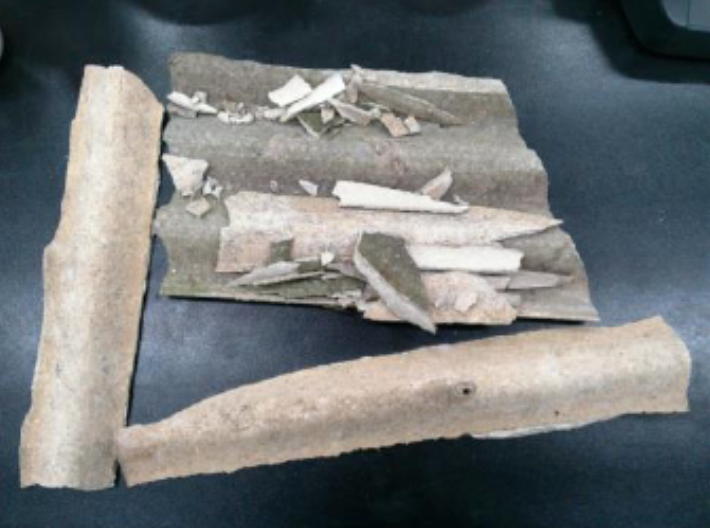
\includegraphics[width=.4\textwidth]{images/chapter2/SamplePrepOne}
}
\subfigure{
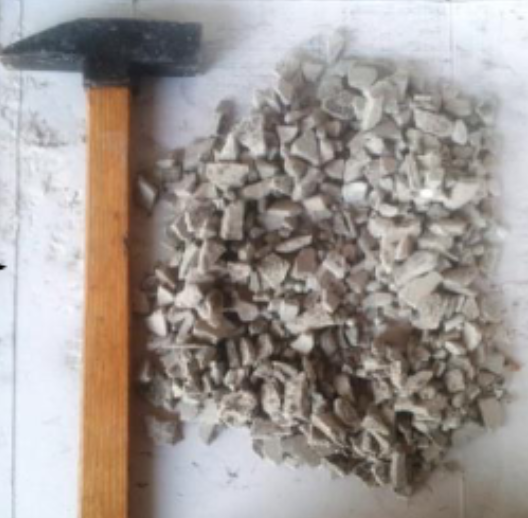
\includegraphics[width=.35\textwidth]{images/chapter2/SamplePrepTwo}
}
\subfigure{
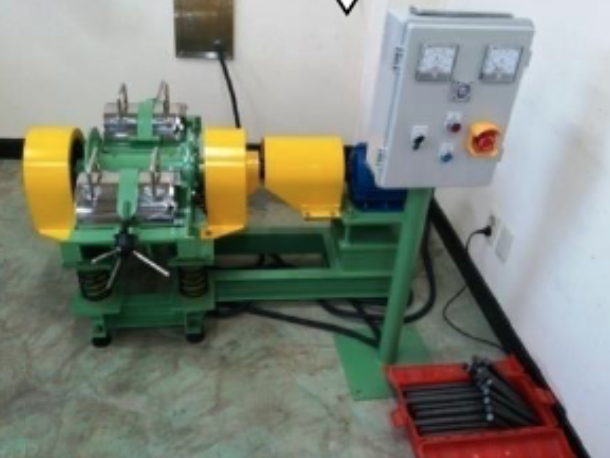
\includegraphics[width=.4\textwidth]{images/chapter2/SamplePrepThree}
}
\subfigure{
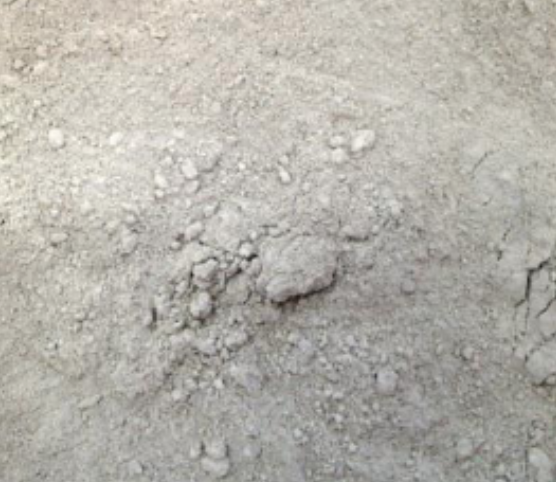
\includegraphics[width=.35\textwidth]{images/chapter2/SamplePrepFour}
}
\label{fig:sampleprep}
\end{figure}


There are many other asbestos detection methods and counting strategies like using certain proteins from Escherichia coli that binds strongly to chrysotile, which in turn makes chrysotile easily detectable with fluorescent microscopy~\cite{kuroda2008detection}. Other current methods are Polarized Light Microscopy (PLM), X-Ray Diffraction (XRD) and Fourier Transform Infrared Spectroscopy (FTIR)~\cite{campopiano2018inter}. In a current and rather big inter-laboratory study, 475 laboratories in Italy were tested if they could reliably detect asbestos fibers in several bulk materials using the above mentioned three methods of PLM, XRD and FTIR. Many laboratories (ranging from 3\% to 40\% depending on the material and asbestos fiber) were classified as unsatisfactory having made too many errors in the classification. The authors concluded that asbestos detection is a complex process that uses several different approaches depending on the material and that the experience and skill of the analyst is very important. Without proper training and a scientific approach, it is very difficult to classify asbestos accurately~\cite{campopiano2018inter}. \\

There are still many other detections methodologies but they all rely on manual screening which is very time-intensive labor. Searching on Google Scholar leads to only a very few papers, that applied some sort of machine learning algorithms in combination with one of the above mentioned microscopy technologies. To the best of my knowledge there has been no work done on the specific combination of SEM and CNN architectures with transfer learning. The only paper that does something similar - using CNN architectures on asbestos images - is from 2018 and has been written by Robson et al.~\cite{robson2018fiac} and is mentioned later on. \\

Cossio et al. describe an unattended scanning electron microscopy analysis with energy dispersive spectrometry (SEM-EDS) for asbestos quantification (counting of the fibers)~\cite{cossio2018innovative}. Their goal was to find an automated process to increase productivity and sensitivity. After having prepared the samples and the SEM images were taken, they needed to be binarized in order to discriminate the shapes clearly from the background. They applied thresholding for that reason and transferred the image from grayscale to a black and white image as seen in Figure~\ref{fig:binarization}.

\begin{figure}[h]
\centering
\caption{Performed binarization on the grayscale image in order to discriminate the asbestos-like structures from the background noise \cite{cossio2018innovative}. }
\subfigure{
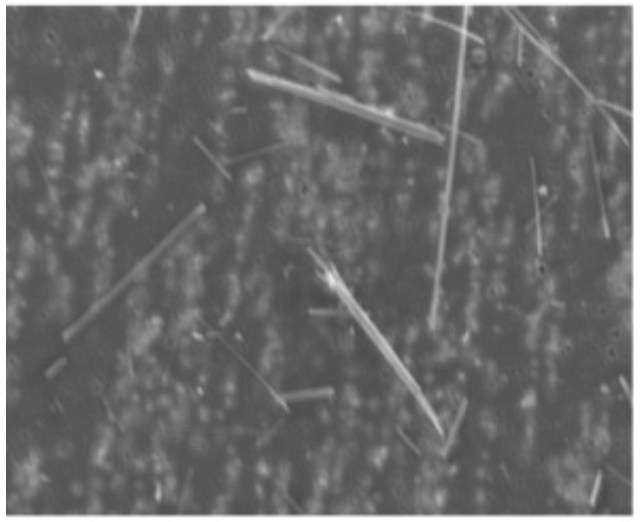
\includegraphics[width=.4\textwidth]{images/chapter2/image_original}
}
\subfigure{
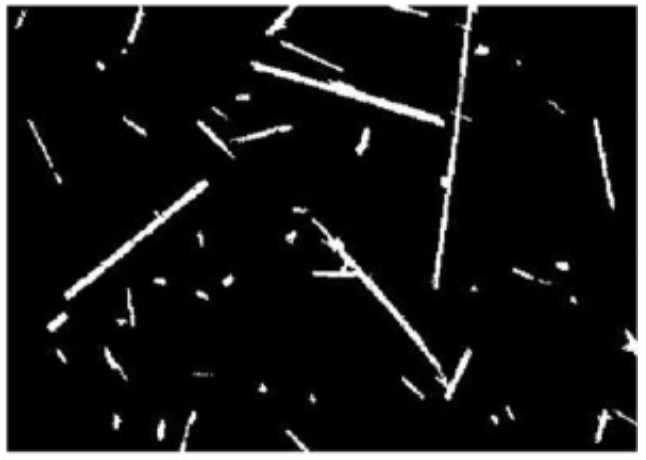
\includegraphics[width=.4\textwidth]{images/chapter2/image_binarized}
}
\label{fig:binarization}
\end{figure}

Then energy dispersive  spectrometry (EDS) is applied on the areas found by image binarization in order to save analytical time. Fiber morphology is then used to analytically discriminate between asbestos fibers and other minerals looking similar to asbestos. That includes length, width and aspect ratio (length/width) of the mineral structure. For the chrysotile fibers, Cossio et al. achieve 49.88\% accuracy in counting the fibers with feret diameters and 78.66\% with equivalent rectangle (ER). Both are morphology methodologies~\cite{cossio2018innovative}.

Kawabata et al. use X-ray diffraction to obtain the image and dispersion staining methods to evaluate and count asbestos-like structures~\cite{kawabata2009asbestos}. The dispersion staining method is a visual inspection in which white light passing through the asbestos structure is dispersed into several colors. For that reason, the fibers need to be immersed into liquid. For chrysotile structures, the dispersion colors are in the range of red-purple to blue. Field interviews revealed that using this method of X-ray diffraction and dispersion staining, no more than 10 samples can be examined daily. The goal of Kawabata et al. was to automate this process by examining color changes of two same images in response to dispersion staining and polarization. Relative to the aspect ratio of the fiber they achieved detection failures (false negatives) of chrysotile fibers in the examined droplets ranging from 0.35 to 0.65, meaning that 35\% to 65\% of the asbestos fibers were missed. The average percentage of incorrectly identified asbestos fibers (false positives) was approximately 20\% for chrysotile~\cite{kawabata2009asbestos}. 

Moriguchi et al. used a similar approach as Kawabate et al. and used the color information from polarization (dispersion) coupled with Support Vector Machine (SVM) as the computer-based detector~\cite{moriguchi2008asbestos}. To get the different properties the sample needs to be captured from two different angles. Since the two images need to be matched, the difference in angle needs to be computationally corrected for. They also found that applying SVM on every single pixel leads to many false positives and false negatives. Therefore they propose to use Conditional Random Field (CRF) on SVM outputs in order to also take the neighboring pixels into account. Miriguchi et al. reach an accuracy of 71\% with the SVM method and 78.9\% with the SVM method coupled with CRF.

Robson et al. developed a method to detect and count asbestos fibers from air samples~\cite{robson2018fiac}. In contrast to soil samples, air samples are much cleaner and have less noise making the detection and counting process more easy and objective. Robson et al. used Mask R-CNN described in~\cite{he2017mask} that adds a mask prediction onto the image itself showing regions that likely include the object of interest. Since Robson et al. had not enough data on hand, data augmentation and transfer learning were also applied. They were able to accurately detect 70\% of the fibers in a test set of 50 images~\cite{robson2018fiac}. \\

\subsubsection{Transfer Learning on Medical Datasets and General SEM Images}

Menegola et al. looked how transfer learning can be applied to a small dataset of melanoma images and improve melanoma detection~\cite{menegola2017knowledge}. They used transfer learning from two distinct datasets. The first dataset is a publicly available medical dataset on diabetic retinopathy detection~\cite{diabeticRetinopathy} and the second dataset is the well known ImageNet~\cite{imagenet}. They found that pre-training on a very general dataset like the ImageNet yields better performance on melanoma detection than pre-training on a similar, medical dataset. They also conclude that fine-tuning the model after transfer learning has been applied leads to better accuracies.

Motlagh et al. have very recently investigated how transfer learning and fine-tuning impacts breast cancer histopathological image classification~\cite{motlagh2018breast}. They used several ResNet and Inception architectures and found consistently better results with ResNet than with Inception. They also concluded that fine-tuning all layers is superior to fine-tuning only the last layer.

There is also a quite recent publication on general SEM image recognition. Modarres et al. have investigated transfer learning techniques on a SEM dataset of roughly 20'000 images and 10 categories~\cite{modarres2017neural}. Their dataset of SEM images is in very high quality showing the objects very clearly. They compared many several different ResNet and Inception architectures and achieved accuracies up to 90\% on the test set. \\


%All in all, it is very difficult to compare the results with each other since every group uses different samples with different pre-processing methods on the image and detection or counting algorithms. It should be noted that none of the mentioned research on asbestos reached an accuracy of 80\% or higher. The publication on general SEM images reached 90\% accuracy but their images were exceptionally clear.\\


\section{Conclusion}

The dataset used in this thesis is very small and classification of certain images is even for humans often difficult or impossible. There is almost no work done on asbestos detection from SEM images in combination with deep learning methods although some publications with rather traditional machine learning approaches were published and introduced in the previous section. Although their methodolgy on asbestos detection cannot be compared with each other, the final results  and accuracies give a good hint on what can be realisticly expected. There are many publications on deep learning with transfer learning applied to medical images that can be considered somewhat similar to the asbestos detection problem. Also, there are publications on deep learning on SEM images in general. There remains much room for further research and evaluation on the combination of deep learning methods with transfer learning on a very small SEM dataset of asbestos.

It should be noted that none of the mentioned research on asbestos reached an accuracy of 80\% or higher. The publication on general SEM images reached 90\% accuracy but their images were exceptionally clear and in perfect quality.\\

















